\chapter{Assignment 7}\label{ass7}

\section{Task 1}\label{ass7_t1}

\subsection{a}\label{ass7_t1a}

In the plots we used three colours to distinguish the results.\\
The blue lines are the current position on the y-axis, the red ones mark the deviation of the yaw and the cyan ones are the control output.\\

Plot for the P-controller with P set to 0.15:\\
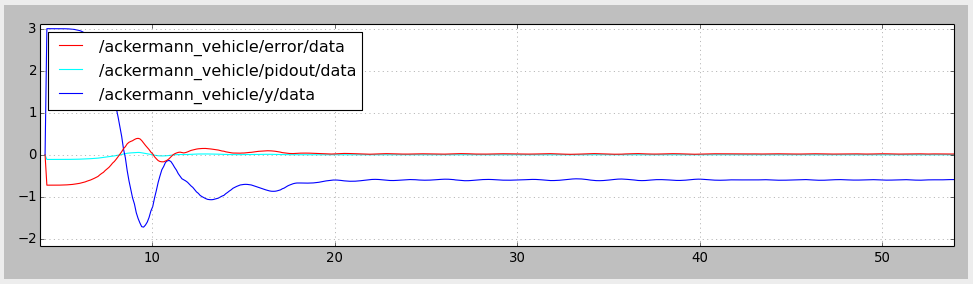
\includegraphics[width=0.75\textwidth]{img/screen_ue7_t1_p-015.png}

Plot for the PD-controller with 0.15(P) and 0.25(D):\\
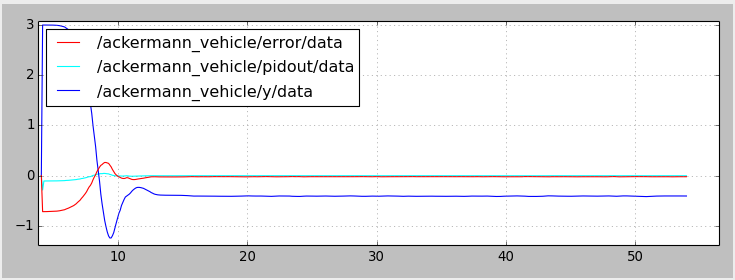
\includegraphics[width=0.75\textwidth]{img/screen_ue7_t1_p-015_d-025.png}

\subsection{b}\label{ass7_t1b}

Plot of P set to 0.05:\\
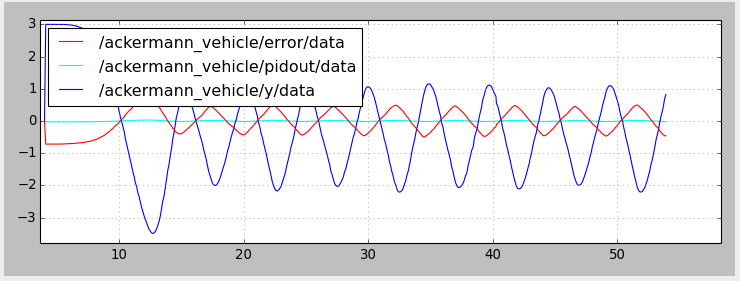
\includegraphics[width=0.75\textwidth]{img/screen_ue7_t2_p-005_osz.png}

As the system starts to oscillate at 0.05 and has a cycle of almost 5, the following equations determine the parameter for the PID-controller:\\
\begin{align*}
K_p &=0.6\cdot K_{p_k}      & = & 0.03\\
K_i &=\frac{2\cdot K_p}{t}  & = & 0.012\\
K_d &=0.12\cdot K_p\cdot t  & = & 0.018
\end{align*}\\

Plot of PID set to 0.03(P), 0.012(I) and 0.018(D):\\
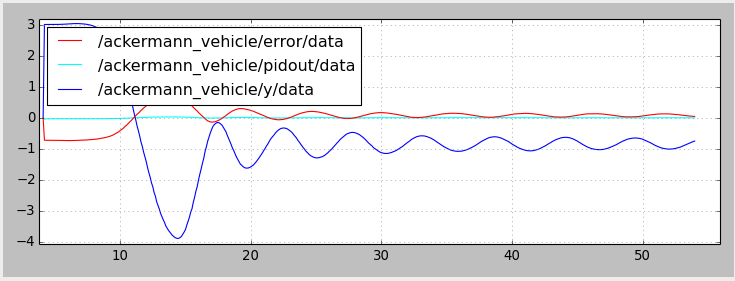
\includegraphics[width=0.75\textwidth]{img/screen_ue7_t2_pid.png}